\newpage
\chapter{METODE PENELITIAN} \label{Bab III}

\section{Alur Penelitian} \label{III.Alur}
Alur penelitian dalam tugas akhir ini divisualisasikan melalui sebuah diagram alir yang menjelaskan setiap tahapan proses penelitian, mulai dari identifikasi masalah hingga tahap akhir penyelesaian. Ilustrasi keseluruhan proses tersebut dapat dilihat pada Gambar 3.1. \par

\begin{figure}[H] % Kalau menggunakan H, posisi gambar akan tepat dibawah teks
    \centering
	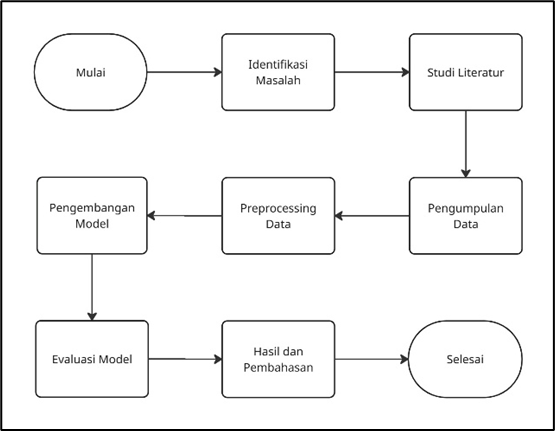
\includegraphics[width=0.6\textwidth]{figure/alur-penelitian.png}
    \caption{Alur Penelitian}
    \label{fig:3.alur}
\end{figure}

\section{Penjabaran Langkah Penelitian} \label{III.Jabar Alur}
Jelaskan secara general langkah-langkah alur penelitian, yang sudah tergambar dalam flowchart di subbab \ref{III.Alur}. Subsubbab berikut harus sesuai dengan jumlah entitas langkah pada alur penelitian. \par

\subsection{Identifikasi Masalah} \label{III.Identifikasi Masalah}
Tahapan identifikasi masalah berfokus pada kerentanan sistem deteksi deepfake di skenario dunia nyata (\textit{in-the-wild}). Sistem deteksi konvensional berbasis analisis spasial statis (\textit{frame-level}) mengalami penurunan akurasi yang signifikan akibat tingginya tingkat realisme manipulasi modern \cite{Cao2022,Lin2025}. Pendekatan alternatif berbasis spatiotemporal (\textit{video-level}) secara teoritis mampu menutupi kelemahan ini dengan mendeteksi anomali gerakan \cite{Gu2021}, namun rentan gagal karena jejak artefak temporal seringkali hancur oleh kompresi tingkat tinggi dan distorsi resolusi pada video nyata \cite{Zi2024,Hsu2020}. Realitas ini memunculkan paradoks empiris di mana penambahan dimensi waktu belum tentu menghasilkan sistem deteksi yang lebih tangguh dibandingkan inspeksi spasial murni \cite{Haliassos2021}. Untuk menjawab kekosongan pembuktian tersebut, penelitian ini merumuskan eksperimen komparatif yang objektif antara arsitektur Vision Transformer (ViT) dan Video Masked Autoencoder (VideoMAE) menggunakan dataset WildDeepfake. \par

\subsection{Studi Literatur} \label{III.Studi Literatur}
Tahap kedua dalam penelitian ini adalah studi literatur, yang mencakup kajian mendalam terhadap berbagai sumber ilmiah yang relevan dengan topik penelitian. Studi literatur ini bertujuan untuk memahami konsep, metode, dan temuan terkini terkait taksonomi manipulasi wajah, kemampuan model deteksi berbasis spasial maupun spatiotemporal, serta karakteristik gangguan pada video deepfake di skenario dunia nyata. Pada tahap ini, ditinjau penelitian yang membahas efektivitas ekstraksi artefak visual statis pada tingkat bingkai tunggal (\textit{frame-level}) \cite{Tolosana2020,Cao2022}, urgensi analisis inkonsistensi gerakan antar-bingkai (\textit{video-level}) \cite{Gu2021}, serta tantangan ekstrem dari proses kompresi media sosial pada dataset WildDeepfake \cite{Zi2024}. Hasil studi literatur tersebut menjadi landasan teoritis untuk merumuskan celah riset pada domain deteksi deepfake dan menyusun rancangan eksperimen komparatif antara arsitektur Vision Transformer (ViT) dan Video Masked Autoencoder (VideoMAE) yang akan dikembangkan dalam penelitian ini. \par

\section{Alat dan Bahan Tugas Akhir} \label{III.Alat dan Bahan}
Berisi alat-alat dan bahan-bahan yang digunakan dalam penelitian. \par

\subsection{Alat} \label{III.Alat}
Alat yang digunakan untuk melakukan penelitian, dapat berupa computer, PC, Arduino, raspberry, etc. Contoh: \par
\begin{enumerate}[noitemsep]
	\item \textit{Notebook} dengan spesifikasi minumum sistem operasi Windows 11, processor AMD Ryzen 5 7430 CPU @ 6 core/2,3 GHz, RAM 16GB DDR4, grafis AMD Radeon RX Vega 7 2GB, SSD 512 GB.
	\item \textit{Smartphone} dengan spesifikasi OS Android OS 12, CPU Snapdragon 778G Octa-core, GPU Adreno 642L, memori 128 GB, RAM 6 GB.
	\item Platform game engine Godot v4.3
	\item Code editor Microsoft Visual Studio Code
	\item Github
\end{enumerate}

\subsection{Bahan} \label{III.Bahan}
Bahan yang digunakan/diperlukan untuk melakukan penelitian, dapat berupa: \par
\begin{enumerate}[noitemsep]
	\item Dataset pihak lain yang diperoleh dengan izin atau dalam lisensi yang diizinkan untuk digunakan secara langsung,
	\item Dataset pihak pertama yang disusun sendiri melalui quisioner, observasi, atau interview,
	\item Dokumen panduan yang mengacu pada standar, hasil tugas akhir, atau artikel yang disitasi dan digunakan. 
\end{enumerate}

\section{Metode Pengembangan} \label{III.Metode}
Membahas mengenai metode yang digunakan dalam penelitian, berdasarkan dasar teori yang sebelumnya sudah dijelaskan pada subbab \ref{II.Teori}. Setiap Tugas Akhir wajib memiliki metode dalam pelaksanaannya yang sesuai dengan penelitian yang dikerjakan: \par
\begin{enumerate}[noitemsep]
	\item Alur pengembangan tugas akhir, menggunakan flowchart
	\item Cara pengumpulan data yang digunakan (Kuesioner, Wawancara, pengujian, dan lainnya)
	\item Metode pengembangan tugas akhir (Metode Waterfall, Agile, RAD, dan lainnya).
	\item Metode pengujian penelitian
\end{enumerate}
Subbab ini akan berhubungan erat dengan Bab \ref{Bab IV}. \par

\section{Ilustrasi Perhitungan Metode} \label{III.Ilustrasi}
Penjelasan contoh perhitungan bagi penelitian tugas akhir yang menggunakan algoritma perhitungan tertentu. Rumus perhitungan berdasarkan rumus yang sudah dijelaskan sebelumnya di Bab \ref{II.Teori}. \par

\section{Rancangan Pengujian} \label{III.Rancang_Uji}
Penjabaran terkait rancangan pengujian, pengujian perangkat keras, lunak, fungsional, dan non-fungsional. Berikan juga hipotesis hasil yang diharapkan dari penelitian. \par
